\documentclass[12pt]{ociamthesis}  % default square logo 
%\documentclass[12pt,beltcrest]{ociamthesis} % use old belt crest logo
%\documentclass[12pt,shieldcrest]{ociamthesis} % use older shield crest logo

%load any additional packages
\usepackage{hyperref}
\usepackage{amssymb}
\usepackage{amsmath}
\usepackage{longtable}
\usepackage{listings} %code listing, memasukkan code

\usepackage{color}
\definecolor{codegreen}{rgb}{0,0.6,0}
\definecolor{codegray}{rgb}{0.5,0.5,0.5}
\definecolor{codepurple}{rgb}{0.58,0,0.82}
\definecolor{backcolour}{rgb}{0.95,0.95,0.92}

\lstdefinestyle{mystyle}{
    backgroundcolor=\color{backcolour},   
    commentstyle=\color{codegreen},
    keywordstyle=\color{magenta},
    numberstyle=\tiny\color{codegray},
    stringstyle=\color{codepurple},
    basicstyle=\footnotesize,
    breakatwhitespace=false,         
    breaklines=true,                 
    captionpos=b,                    
    keepspaces=true,                 
    numbers=left,                    
    numbersep=5pt,                  
    showspaces=false,                
    showstringspaces=false,
    showtabs=false,                  
    tabsize=2,
    language=sh
}
\lstset{style=mystyle}
%input macros (i.e. write your own macros file called mymacros.tex 
%and uncomment the next line)
%\include{mymacros}

\title{Panduan Cara\\[1ex]     %your thesis title,
        Penggunaan Kepo }   %note \\[1ex] is a line break in the title

\author{\begin{tabular}[t]{l@{\extracolsep{1em}}l} 
Rolly Maulana Awangga  & \textbf{github.com/awangga} \\
Syafrial Fachri Pane & \textbf{github.com/fachrie007} \\
Muhammad Wahyu Ardi Ismail & \textbf{github.com/wahyuardi}\\
Dinda Majesty & \textbf{github.com/dindamajesty13}\\
Tri Angga Dio Simamora & \textbf{github.com/trianggadios}
\end{tabular}
}             %your name
\college{}  %your college

%\renewcommand{\submittedtext}{change the default text here if needed}
\degree{Applied Bachelor Program of Informatics Engineering}     %the degree
\degreedate{Bandung\\ 2019}         %the degree date

%end the preamble and start the document
\begin{document}

%this baselineskip gives sufficient line spacing for an examiner to easily
%markup the thesis with comments
\baselineskip=18pt plus1pt

%set the number of sectioning levels that get number and appear in the contents
\setcounter{secnumdepth}{3}
\setcounter{tocdepth}{3}


\maketitle                  % create a title page from the preamble info
\begin{dedication}
`Jika Kamu tidak dapat menahan lelahnya belajar, \\
Maka kamu harus sanggup menahan perihnya Kebodohan.'\\ 
~Imam Syafi'i~\\
\end{dedication}        % include a dedication.tex file
\begin{acknowledgements}
Puji dan syukur kami panjatkan hadirat Allah S.W.T atas rahmat dan karunia-Nya kami dapat menyelesaikan panduan cara penggunaan kepo.
Dan tidak lupa juga kami ucapkan kepada rekan dan para dosen yang namanya tidak dapat kami sebutkan satu per satu, yang telah membantu kami dalam proses pengerjaan panduan cara penggunaan kepo ini, diharapkan panduan ini dapat berguna bagi para pembaca dan juga menjadi acuan dalam menggunakan program kepo.
\end{acknowledgements}   % include an acknowledgements.tex file
\begin{abstract}
	Panduan Cara Penggunan Kepo ini dibuat dengan tujuan memberikan pemahaman mendalam tentang penggunaan program kepo kepada para sivitas akademika. Dengan demikian diharapkan semua sivitas akademika dapat melakukan aktivitas atau kegiatan dengan lancar dan sesuai standar.

\end{abstract}          % include the abstract

\begin{romanpages}          % start roman page numbering
\tableofcontents            % generate and include a table of contents         

\listoffigures

\end{romanpages}            % end roman page numbering

%now include the files of latex for each of the chapters etc
\chapter{Kepo}
Kepo atau \textit{Key Production} adalah sebuah program yang digunakan pada proyek 2 dan proyek 3, berfungsi untuk memudahkan mahasiswa untuk malakukan bimbingan disetiap pertemuan. Kepo menggunakan bahasa pemrograman Python, dan terhubung dengan github melalui repositori dari masing-masing \textit{user}.


\section{Cara Menggunakan Kepo}
\par Cara menggunakan program kepo yaitu:

\begin{enumerate}
\item Langkah pertama buka url if.poltekpos.ac.id jika sudah kemudian klik \textit{read more}.

 \begin{figure}[!htbp]
    \centering
    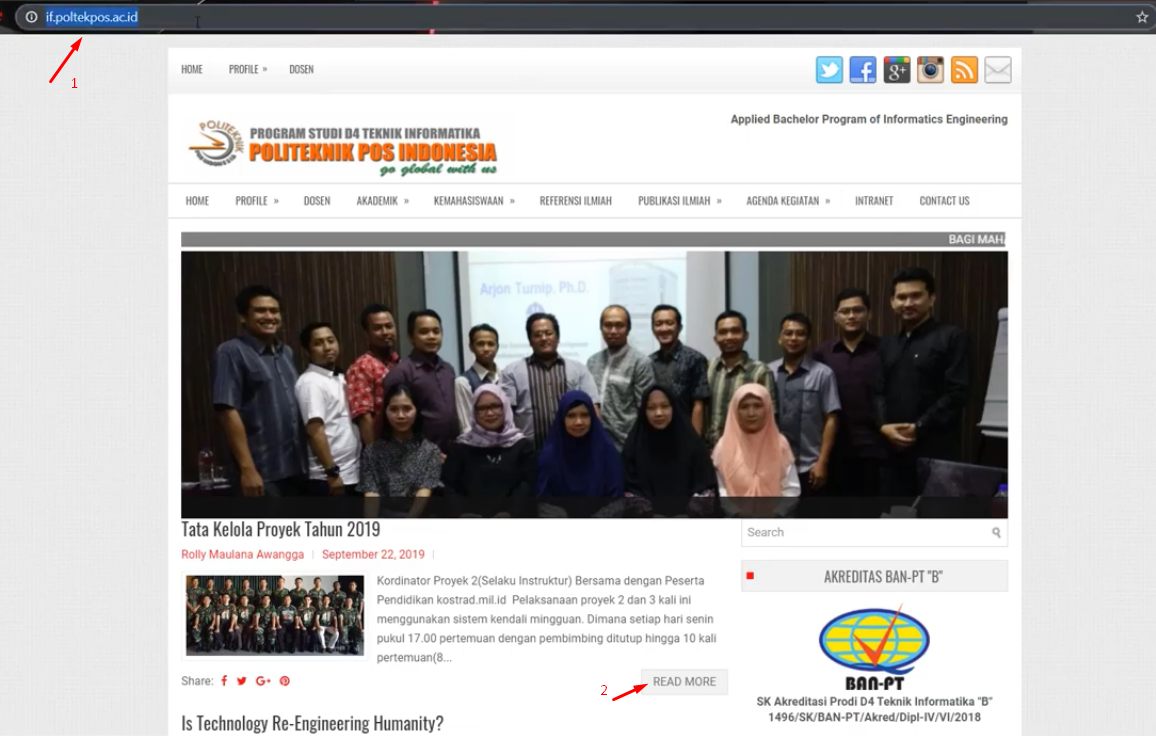
\includegraphics[width=10cm]{figures/if}
    \caption{\textit{Tampilan if.poltekpos.ac.id}}
    
\end{figure} 

\newpage

\item kemudian klik kepo
\begin{figure}[!htbp]
    \centering
    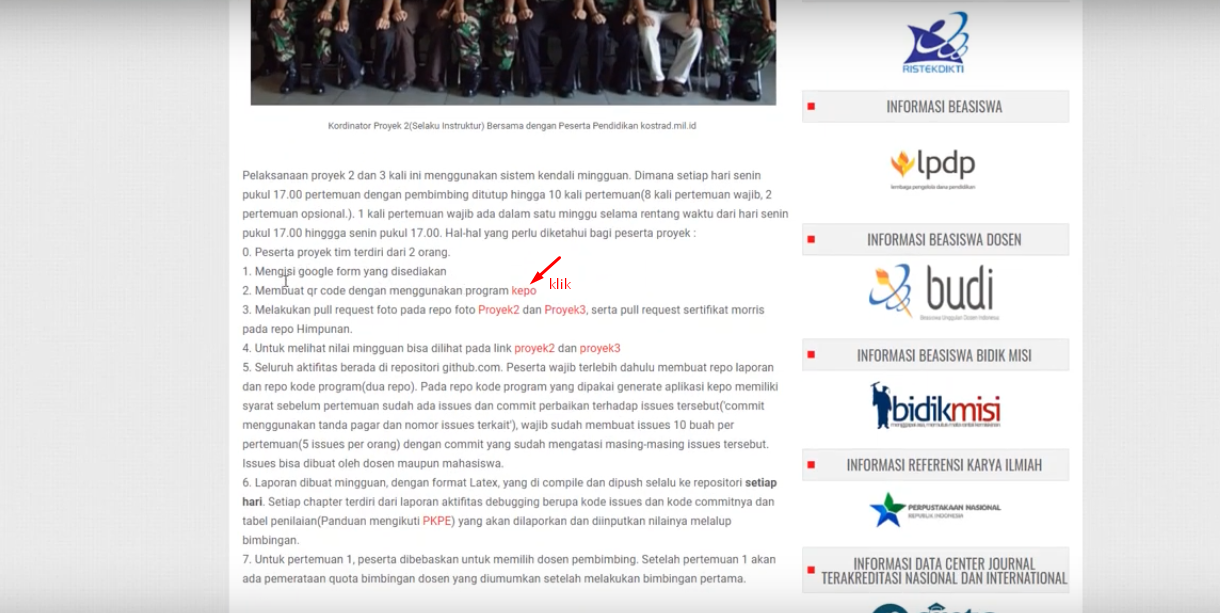
\includegraphics[width=10cm]{figures/klikkepo}
    \caption{\textit{klik kepo}}
    
\end{figure} 

atau bisa juga dengan membuka url https://github.com/awangga/kepo

\begin{figure}[!htbp]
    \centering
    
\includegraphics[width=10cm]{figures/kepo}
    \caption{\textit{membuka kepo melalui url}}
\end{figure} 


\item kemudian klik \textit{fork}, jika sudah \textit{clone or download}, atau \textit{download zip}.

\begin{figure}[!htbp]
    \centering
    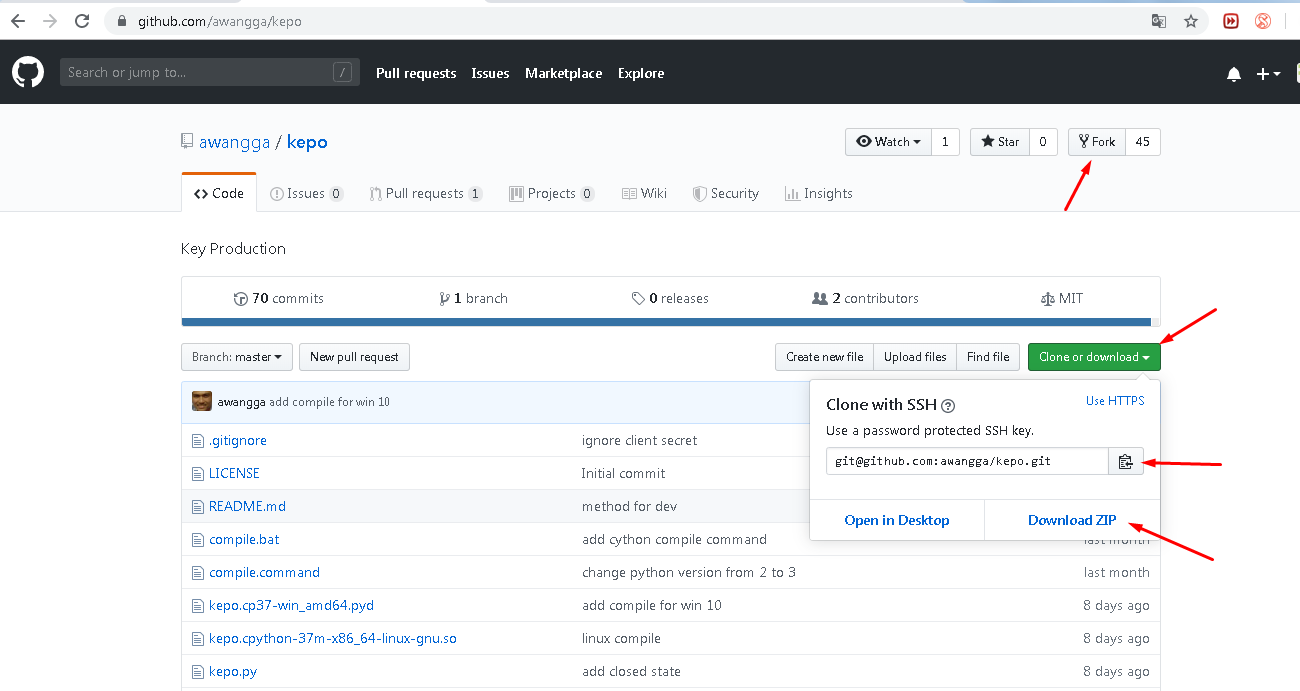
\includegraphics[width=13cm]{figures/tutor}
    \caption{\textit{mendownload kepo}}
\end{figure} 

\newpage

\item buka folder kepo, kemudian \textit{rename} kepo.cp37-winamd64  menjadi kepo.py 
\begin{figure}[!htbp]
    \centering
    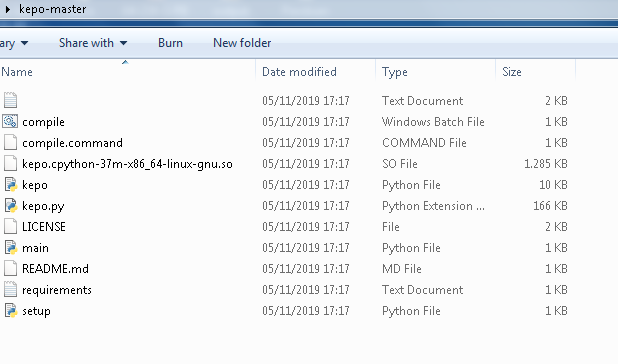
\includegraphics[width=10cm]{figures/rename}
    \caption{\textit{rename}}
\end{figure} 

\item kemudian buka github, lalu buat repo baru. Jika program menggunakan bahasa pemrograman python, pilih python, pada \textit{add a license} pilih MIT license, jika sudah klik \textit{create new repository}.

\begin{figure}[!htbp]
    \centering
    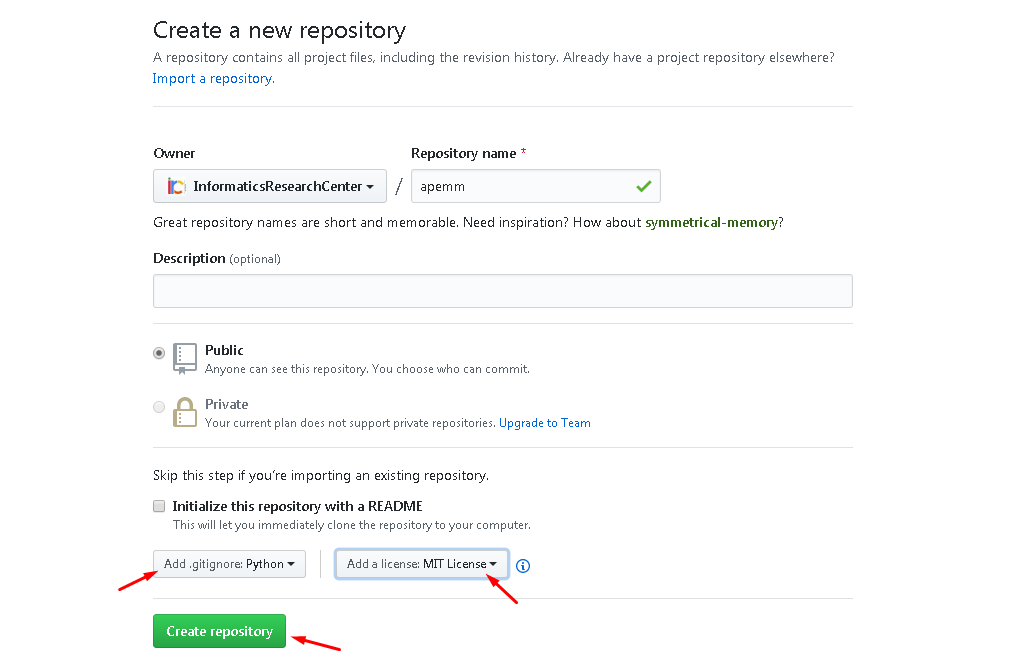
\includegraphics[width=13cm]{figures/newrepo}
    \caption{\textit{create new repository}}
\end{figure} 

\newpage

\item buat 10 \textit{issues} terlebih dahulu.

\begin{figure}[!htbp]
    \centering
    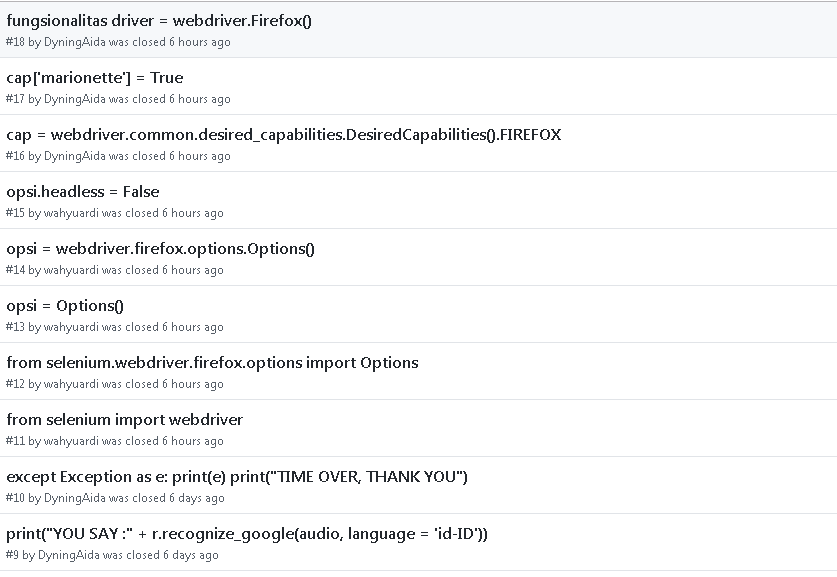
\includegraphics[width=10cm]{figures/issues}
    \caption{\textit{membuat 10 issues}}
\end{figure} 

\item setelah itu \textit{download chrome driver}sesuai versi chrome yang digunakan.

\begin{figure}[!htbp]
    \centering
    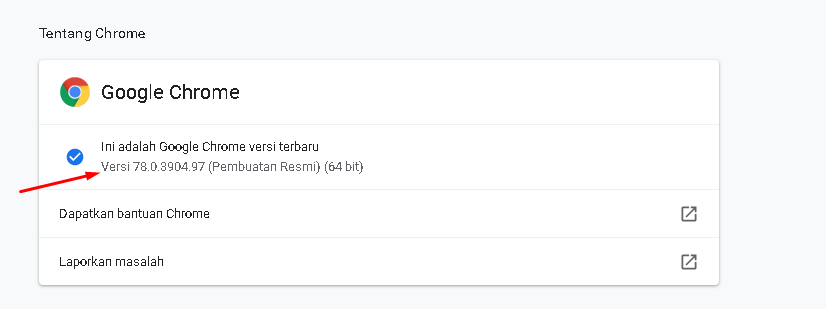
\includegraphics[width=10cm]{figures/versichrome}
    \caption{\textit{versi chrome}}
\end{figure} 

\begin{figure}[!htbp]
    \centering
    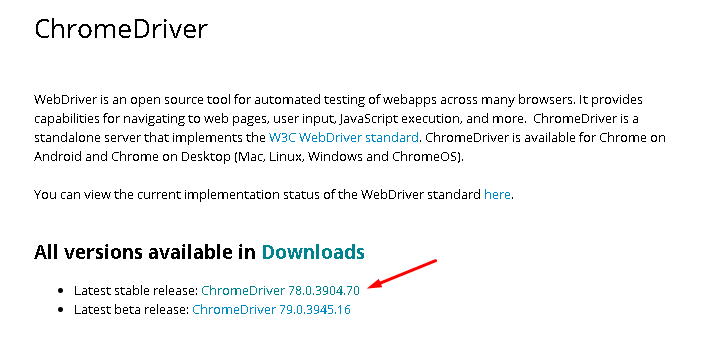
\includegraphics[width=10cm]{figures/chromedriver}
    \caption{\textit{chrome driver}}
\end{figure} 

\newpage

\item letakkan \textit{chrome driver} ke windows-system32

\begin{figure}[!htbp]
    \centering
    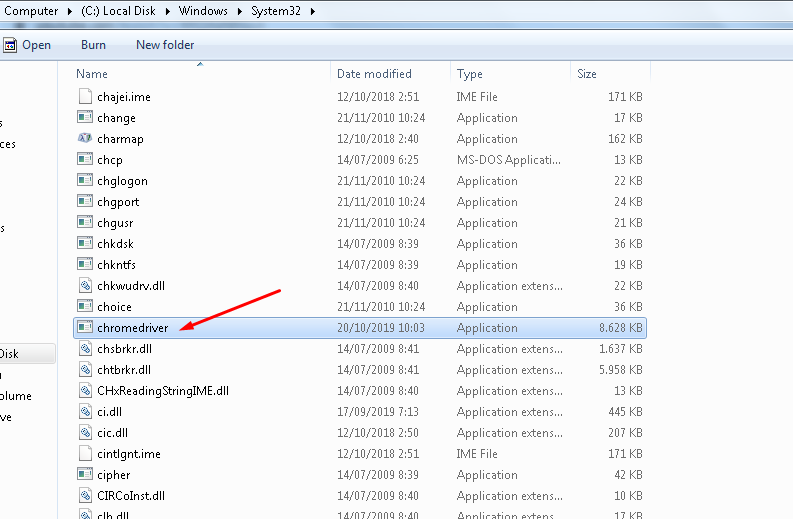
\includegraphics[width=10cm]{figures/pindahchrome}
    \caption{\textit{pindahkan chrome driver ke windows system32}}
\end{figure} 

\item kemudian buka folder kepo, lalu pada ketik CMD untuk mempermudah.

\begin{figure}[!htbp]
    \centering
    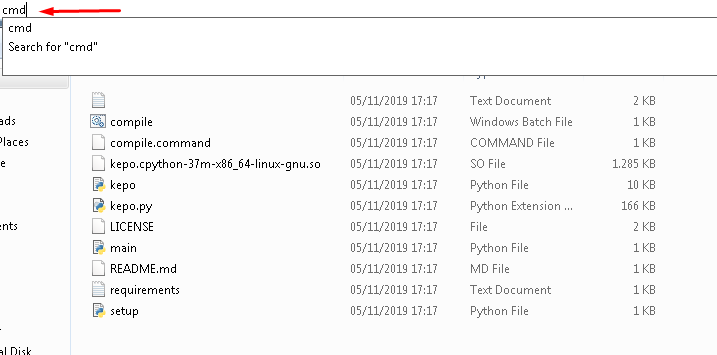
\includegraphics[width=10cm]{figures/folderkepo}
    \caption{\textit{membuka folder kepo}}
\end{figure} 

\newpage

\item pada cmd ketikkan perintah pip install -r requirements.txt dan
python main.py

\begin{figure}[!htbp]
    \centering
    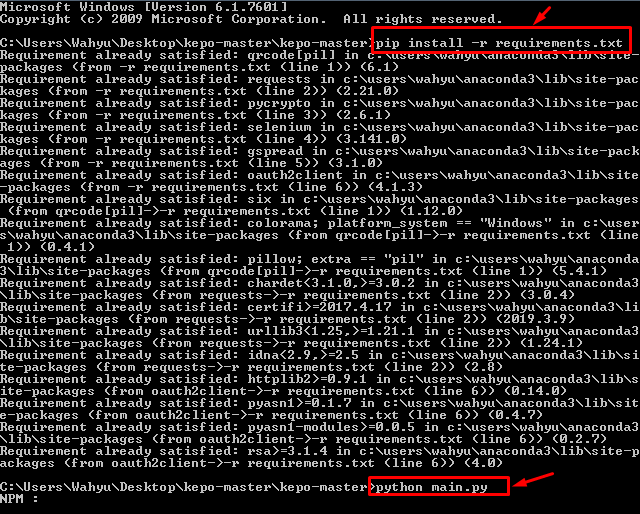
\includegraphics[width=10cm]{figures/cmd}
    \caption{\textit{cmd}}
\end{figure}

\item kemudian \textit{input} 

\begin{figure}[!htbp]
    \centering
    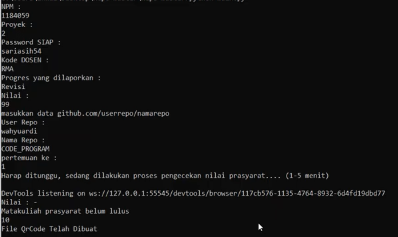
\includegraphics[width=10cm]{figures/inputt}
    \caption{\textit{input}}
\end{figure}

\newpage

\item qrcode akan muncul di folder kepo

\begin{figure}[!htbp]
    \centering
    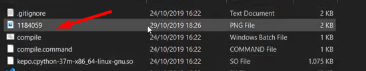
\includegraphics[width=10cm]{figures/qrcode}
    \caption{\textit{file qrcode}}
\end{figure}

kemudian klik file qrcodenya, dan ini adalah qrcode tersebut.
\begin{figure}[!htbp]
    \centering
    
\includegraphics[width=10cm]{figures/iniqrcode}
    \caption{\textit{qrcode}}
\end{figure}

\end{enumerate}

\newpage

\subsection{Jika issues kurang dari 10}
\par jika \textit{issues} kurang dari 10 maka :

\begin{figure}[!htbp]
    \centering
    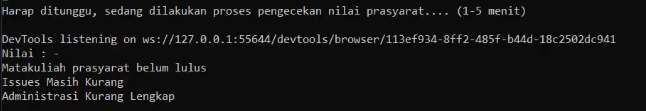
\includegraphics[width=15cm]{figures/issueskurang}
    \caption{\textit{issues kurang dari 10}}
\end{figure}


\chapter{Commit}

\section{Cara Commit}
\par cara \textit{commit issues} yaitu :

\begin{enumerate}
\item Langkah pertama dengan membuka file yang diletakkan di LocalDisk C-users-namafolder 

\begin{figure}[!htbp]
    \centering
    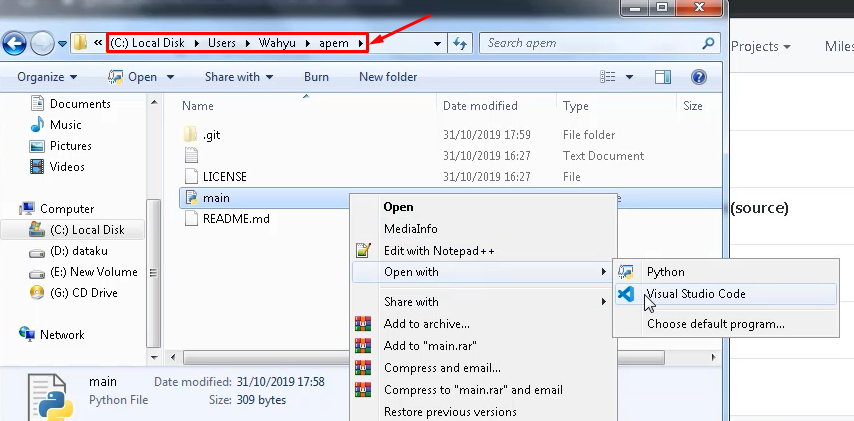
\includegraphics[width=7cm]{figures/file}
    \caption{\textit{file yang akan dicommit}}
\end{figure}

\item kemudian buat tanda "\# issues" untuk menandakan codingan yang terdapat \textit{error}. contoh \textit{error} karena identasi.

\begin{figure}[!htbp]
    \centering
    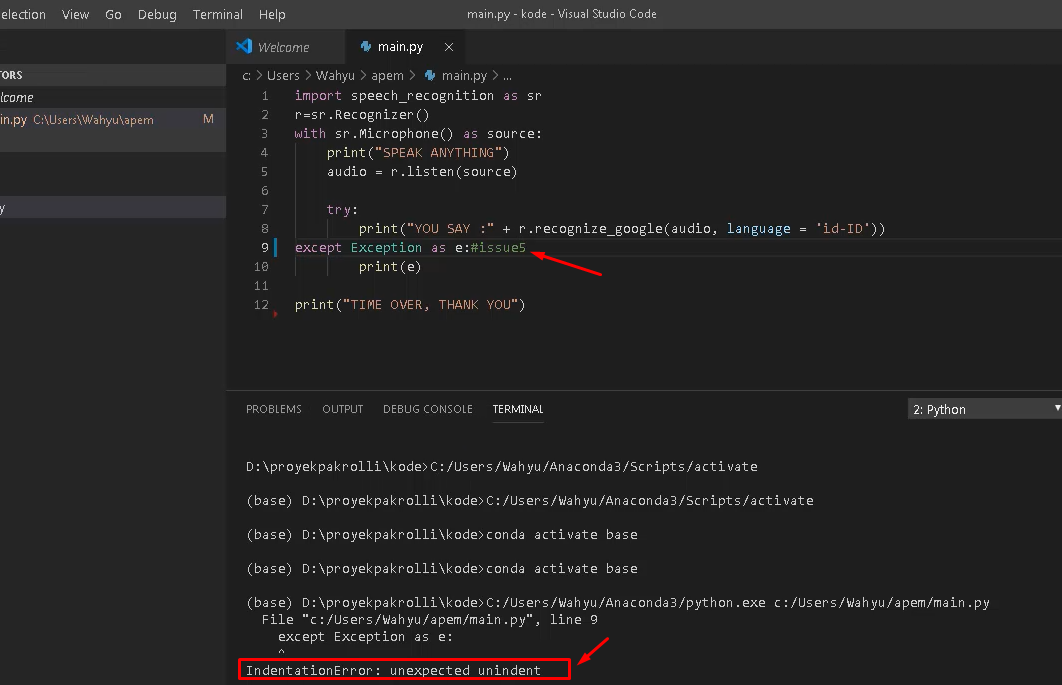
\includegraphics[width=7cm]{figures/error}
    \caption{\textit{error karena identasi}}
\end{figure}

\newpage

\item kemudian buka file yang diletakkan di LocalDiskC-users-namafolder. Kemudian klik kanan pada mouse, kemudian kik \textit{Git Bash here}

\begin{figure}[!htbp]
    \centering
    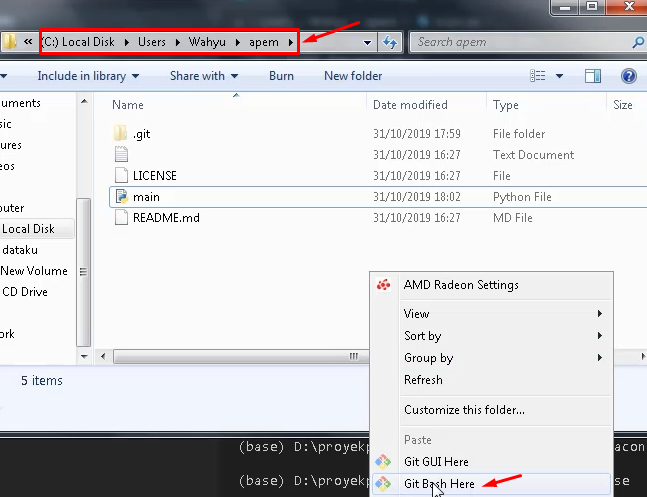
\includegraphics[width=10cm]{figures/bukafolder}
    \caption{\textit{Git Bash here}}
\end{figure}

\item Kemudian ketik

\begin{figure}[!htbp]
    \centering
    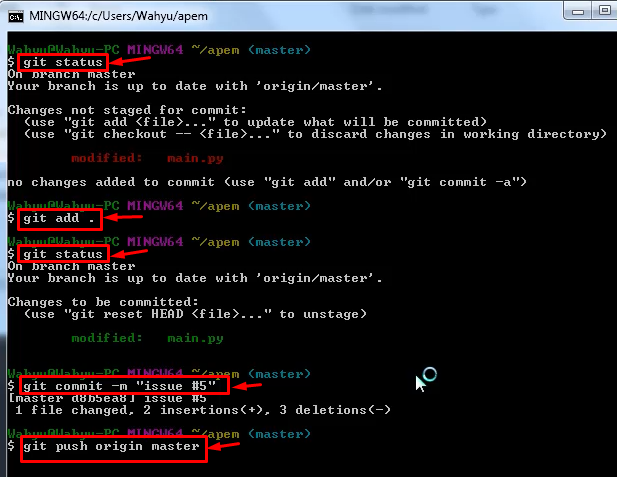
\includegraphics[width=12cm]{figures/git}
    \caption{\textit{cara commit issues}}
\end{figure}

\newpage

\item Kemudian menangani \textit{error} pada codingan, dan beri komentar dengan "\# penyelesaian issues"

\begin{figure}[!htbp]
    \centering
    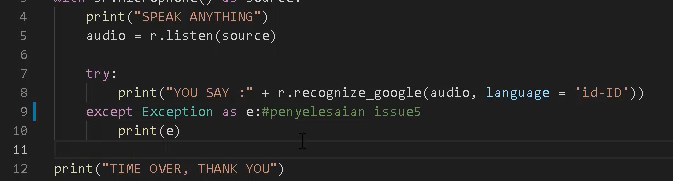
\includegraphics[width=10cm]{figures/atasi}
    \caption{\textit{menangatasi error}}
\end{figure}

\item Buka file yang diletakkan di LocalDiskC-users-namafolder. Kemudian klik kanan pada mouse, kemudian kik \textit{Git Bash here}

\begin{figure}[!htbp]
    \centering
    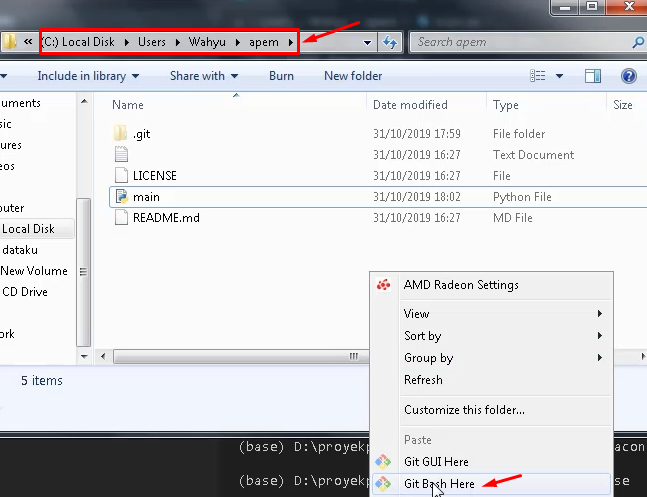
\includegraphics[width=10cm]{figures/bukafolder}
    \caption{\textit{Git Bash here}}
\end{figure}

\newpage

\item kemudian ketik pada cmd

\begin{figure}[!htbp]
    \centering
    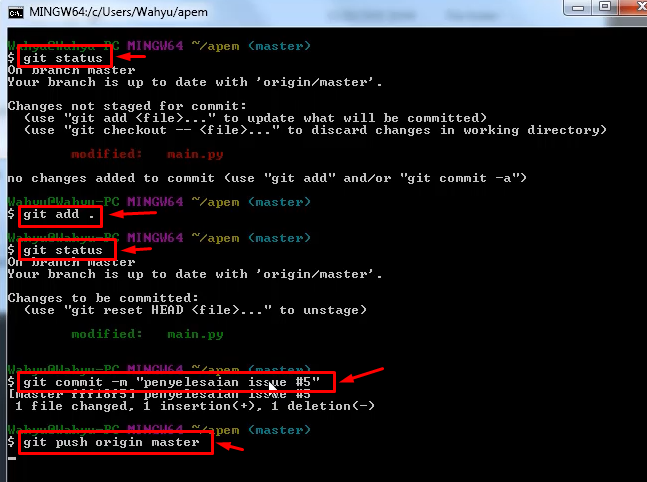
\includegraphics[width=10cm]{figures/ketik}
    \caption{\textit{cara commit issues}}
\end{figure}

\item Buka \textit{issues} yang tadi telah di \textit{commit}, tampilannya seperti ini:

\begin{figure}[!htbp]
    \centering
    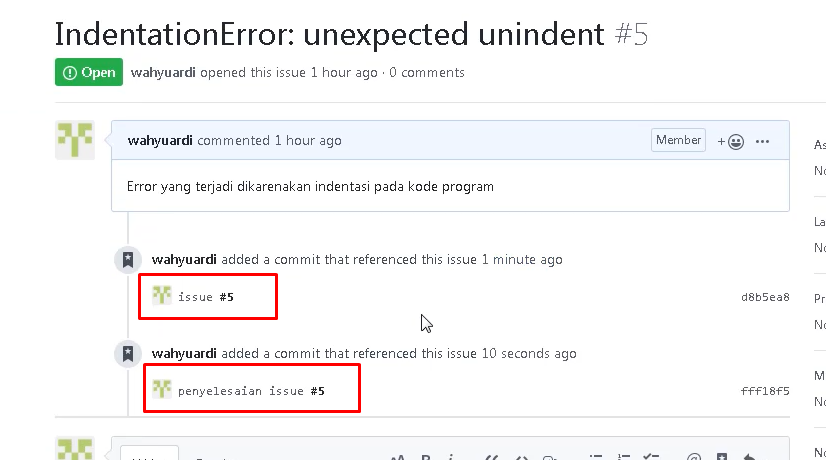
\includegraphics[width=10cm]{figures/errordanpenaganan}
    \caption{\textit{issues error dan issues penyelesaian}}
\end{figure}

\newpage

\item Tampilan \textit{issues error}
\begin{figure}[!htbp]
    \centering
    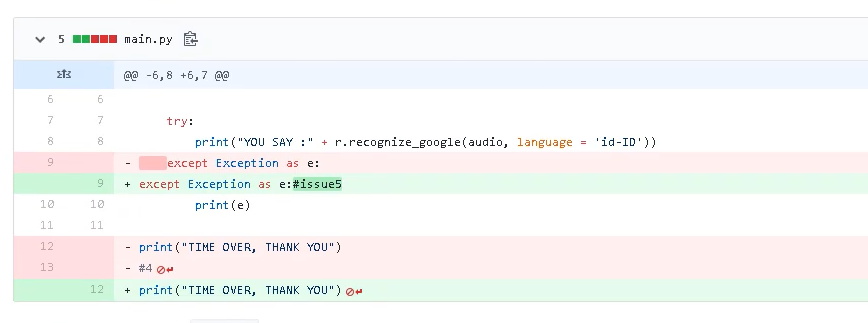
\includegraphics[width=12cm]{figures/tampilanissueserror}
    \caption{\textit{tampilan issues error}}
\end{figure}

\item Tampilan \textit{issues} penyelesaian
\begin{figure}[!htbp]
    \centering
    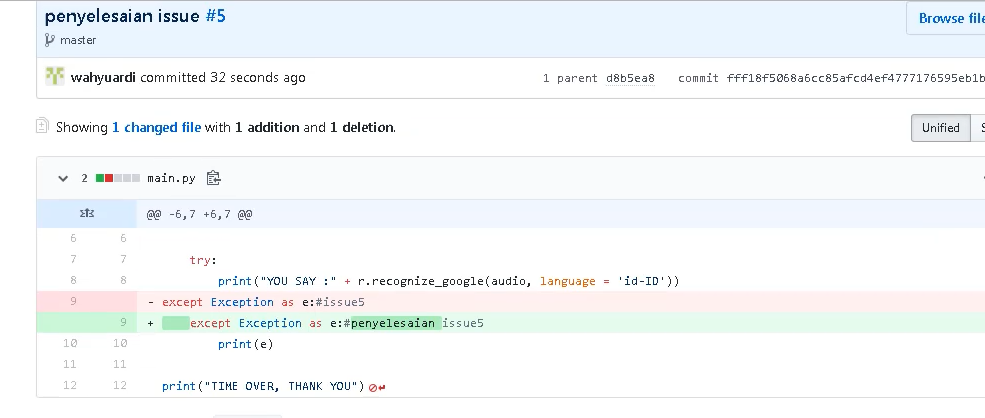
\includegraphics[width=12cm]{figures/tampilanissuespenyelesaian}
    \caption{\textit{tampilan issues penyelesaian}}
\end{figure}

\end{enumerate}



%now enable appendix numbering format and include any appendices
%\appendix
%\chapter{Latex Symbol}
Berikut adalah daftar pemakaian simbol dalam latex
\begin{enumerate}
	\item The Comprehensive LATEX Symbol List : \\
	\verb|http://tug.ctan.org/info/symbols/comprehensive/symbols-a4.pdf|
	\item List of Math Symbol : \\
	\verb|https://oeis.org/wiki/List_of_LaTeX_mathematical_symbols|
	\item List of Latex Symbol : \\
	\verb|http://latex.wikia.com/wiki/List_of_LaTeX_symbols|
\end{enumerate}
%\chapter{Contoh Penilaian Reviewer Jurnal}

gambar \ref{form1} dan \ref{form2} merupakan contoh bagaimana reviewer menilai jurnal kita. 
\begin{figure}[ht]
      \centerline{\includegraphics[width=1\textwidth]
      {figures/form1}}
      \caption{Form nilai bagian 1.}
      \label{form1}
      \end{figure}

	\begin{figure}[ht]
	      \centerline{\includegraphics[width=1\textwidth]
	      {figures/form2}}
	      \caption{form nilai bagian 2.}
	      \label{form2}
	      \end{figure}


%next line adds the Bibliography to the contents page
\addcontentsline{toc}{chapter}{Bibliography}
%uncomment next line to change bibliography name to references
%\renewcommand{\bibname}{References}
\bibliography{references}        %use a bibtex bibliography file refs.bib
\bibliographystyle{plain}  %use the plain bibliography style

\end{document}

